\message{ !name(thesis.tex)}\documentclass[12pt,letterpaper]{report}
%
% Review cuthesis.sty for more documentation on available options
% for this package.

% Leave the below option as "masters," as it generates "thesis" on title page. 
% PhD generates "dissertation" and that word is not recognized by Carleton Library
\usepackage[masters,2committee]{cuthesis}
\usepackage{array}
\usepackage{graphicx}
\usepackage{cite}
\usepackage{subfigure}
\usepackage{amsmath}
\usepackage[indent,bf]{caption}
\usepackage{rotating}
\usepackage{setspace}
\usepackage{longtable}
\usepackage{rotating}




% Defines relative path to folder containing your figures
\graphicspath{{figures/}}
\providecommand{\norm}[1]{\lvert#1\rvert} 

\begin{document}

\message{ !name(chapter6.tex) !offset(475) }
\begin{figure}[h]
  \centering
  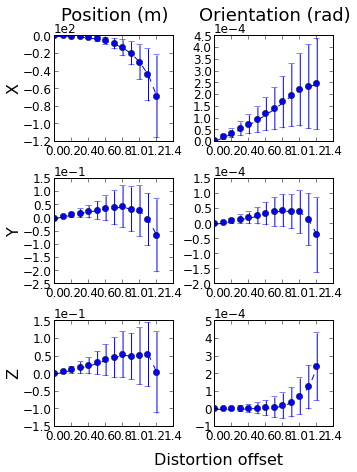
\includegraphics[width=10cm,keepaspectratio=true]{./Figures/SimulationFigures/Figure47.png}
  \caption{UAS localization error with lens distortion}
  \label{fig:simfig47}
\end{figure}

\begin{figure}[h]
  \centering
  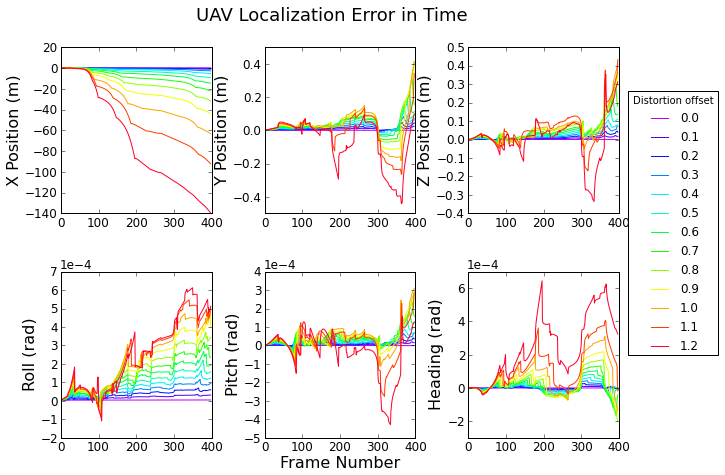
\includegraphics[width=10cm,keepaspectratio=true]{./Figures/SimulationFigures/Figure48.png}
  \caption{UAS localization error with lens distortion plotted against frame number}
  \label{fig:simfig48}
\end{figure}


%%% Local Variables:
%%% mode: latex
%%% TeX-master: "thesis"
%%% End:





\message{ !name(thesis.tex) !offset(47) }

\end{document}

%%% Local Variables: 
%%% mode: latex
%%% TeX-master: t
%%% End: 
